\documentclass[12pt]{article}

% Load CFES common styles
\usepackage{../../shared/styles/cfes-common}
\usepackage{../../shared/styles/cfes-headers}
\usepackage{../../shared/styles/ninecolors}

% Stance-specific helpers
% Shared helpers for the Cahier des positions (French Document of Stances).
% Included by main.tex (combined build) and by each standalone driver.
%
% Styling mirrors the original .docx: a CFES blue accent, unnumbered section
% titles and subheadings each underlined by a thin rule, a borderless
% left/right adoption table, a lightly-boxed blue official-stance statement,
% and justified body text.

\RequirePackage{xcolor}
\RequirePackage{titlesec}

% CFES blue sampled from the source document.
\definecolor{cfesblue}{HTML}{275D9F}

% No coloured/boxed borders around hyperlinks or TOC entries.
\hypersetup{hidelinks}

% --- Section titles -------------------------------------------------------
% Unnumbered, CFES blue, followed by a full-width rule. Still listed in the
% table of contents.
\titleformat{\section}
  {\normalfont\Large\bfseries\color{cfesblue}}
  {}
  {0pt}
  {}
  [{\vspace{2pt}\color{cfesblue}\titlerule[0.8pt]}]
\titlespacing*{\section}{0pt}{*2}{*1.2}

% Drop section numbering entirely (titles are unnumbered) while keeping the
% counter stepping so labels/refs still work.
\setcounter{secnumdepth}{0}

% --- Adoption / revision metadata ----------------------------------------
% Borderless, "Adopté:" flush left and "Dernière mise à jour:" flush right,
% headings in blue with the values on the line below.
% Usage: \stanceinfo{Adopted text}{Last updated text}
\newcommand{\stanceinfo}[2]{%
 \par\vspace{0.3em}%
 \noindent
 \begin{minipage}[t]{0.5\textwidth}
  {\color{cfesblue}\textbf{Adopté:}}\\[2pt]#1
 \end{minipage}%
 \begin{minipage}[t]{0.5\textwidth}
  \raggedleft
  {\color{cfesblue}\textbf{Dernière mise à jour:}}\\[2pt]#2
 \end{minipage}%
 \par\vspace{0.6em}%
}

% --- Official stance ------------------------------------------------------
% Blue statement text inside a thin single-rule frame.
% Usage: \officialstance{statement text}
\newcommand{\officialstance}[1]{%
 \par\vspace{0.2em}%
 \noindent\textit{La position officielle:}\par
 \vspace{0.4em}%
 \noindent
 \fcolorbox{cfesblue}{white}{%
  \begin{minipage}{\dimexpr\textwidth-2\fboxsep-2\fboxrule\relax}
   \color{cfesblue}\textbf{#1}
  \end{minipage}%
 }%
 \par\vspace{0.7em}%
}

% --- Subheadings ----------------------------------------------------------
% CFES blue, bold, underlined by a thin full-width rule.
% Usage: \stanceheading{La position des étudiants}
\newcommand{\stanceheading}[1]{%
 \par\vspace{0.7em}%
 {\noindent\bfseries\color{cfesblue}#1}%
 \par\vspace{1pt}{\color{cfesblue}\titlerule[0.5pt]}%
 \par\vspace{0.4em}%
}


\begin{document}

% Title page
\begin{tikzpicture}[remember picture,overlay]
 % Top image (image2.png)
 \node[anchor=north west, inner sep=0pt] at (current page.north west) {
  
\includegraphics[width=\paperwidth]{../../shared/assets/media/image2.png}
 };

 % Middle text content
 \node[anchor=center] at (current page.center) {
  \begin{minipage}{0.8\textwidth}
   \centering
   % Organization name (font size 12)
   {\fontsize{12}{14}\selectfont La Fédération canadienne étudiante en génie}

   \vspace{1cm}

   % Document title (font size 48)
   {\fontsize{48}{58}\selectfont \textbf{Cahier des positions}}

   \vspace{1cm}

   % Edition text (font size 12)
   {\fontsize{12}{14}\selectfont Édition française}
  \end{minipage}
 };

 % Bottom image (image3.png)
 \node[anchor=south west, inner sep=0pt] at (current page.south west) {
  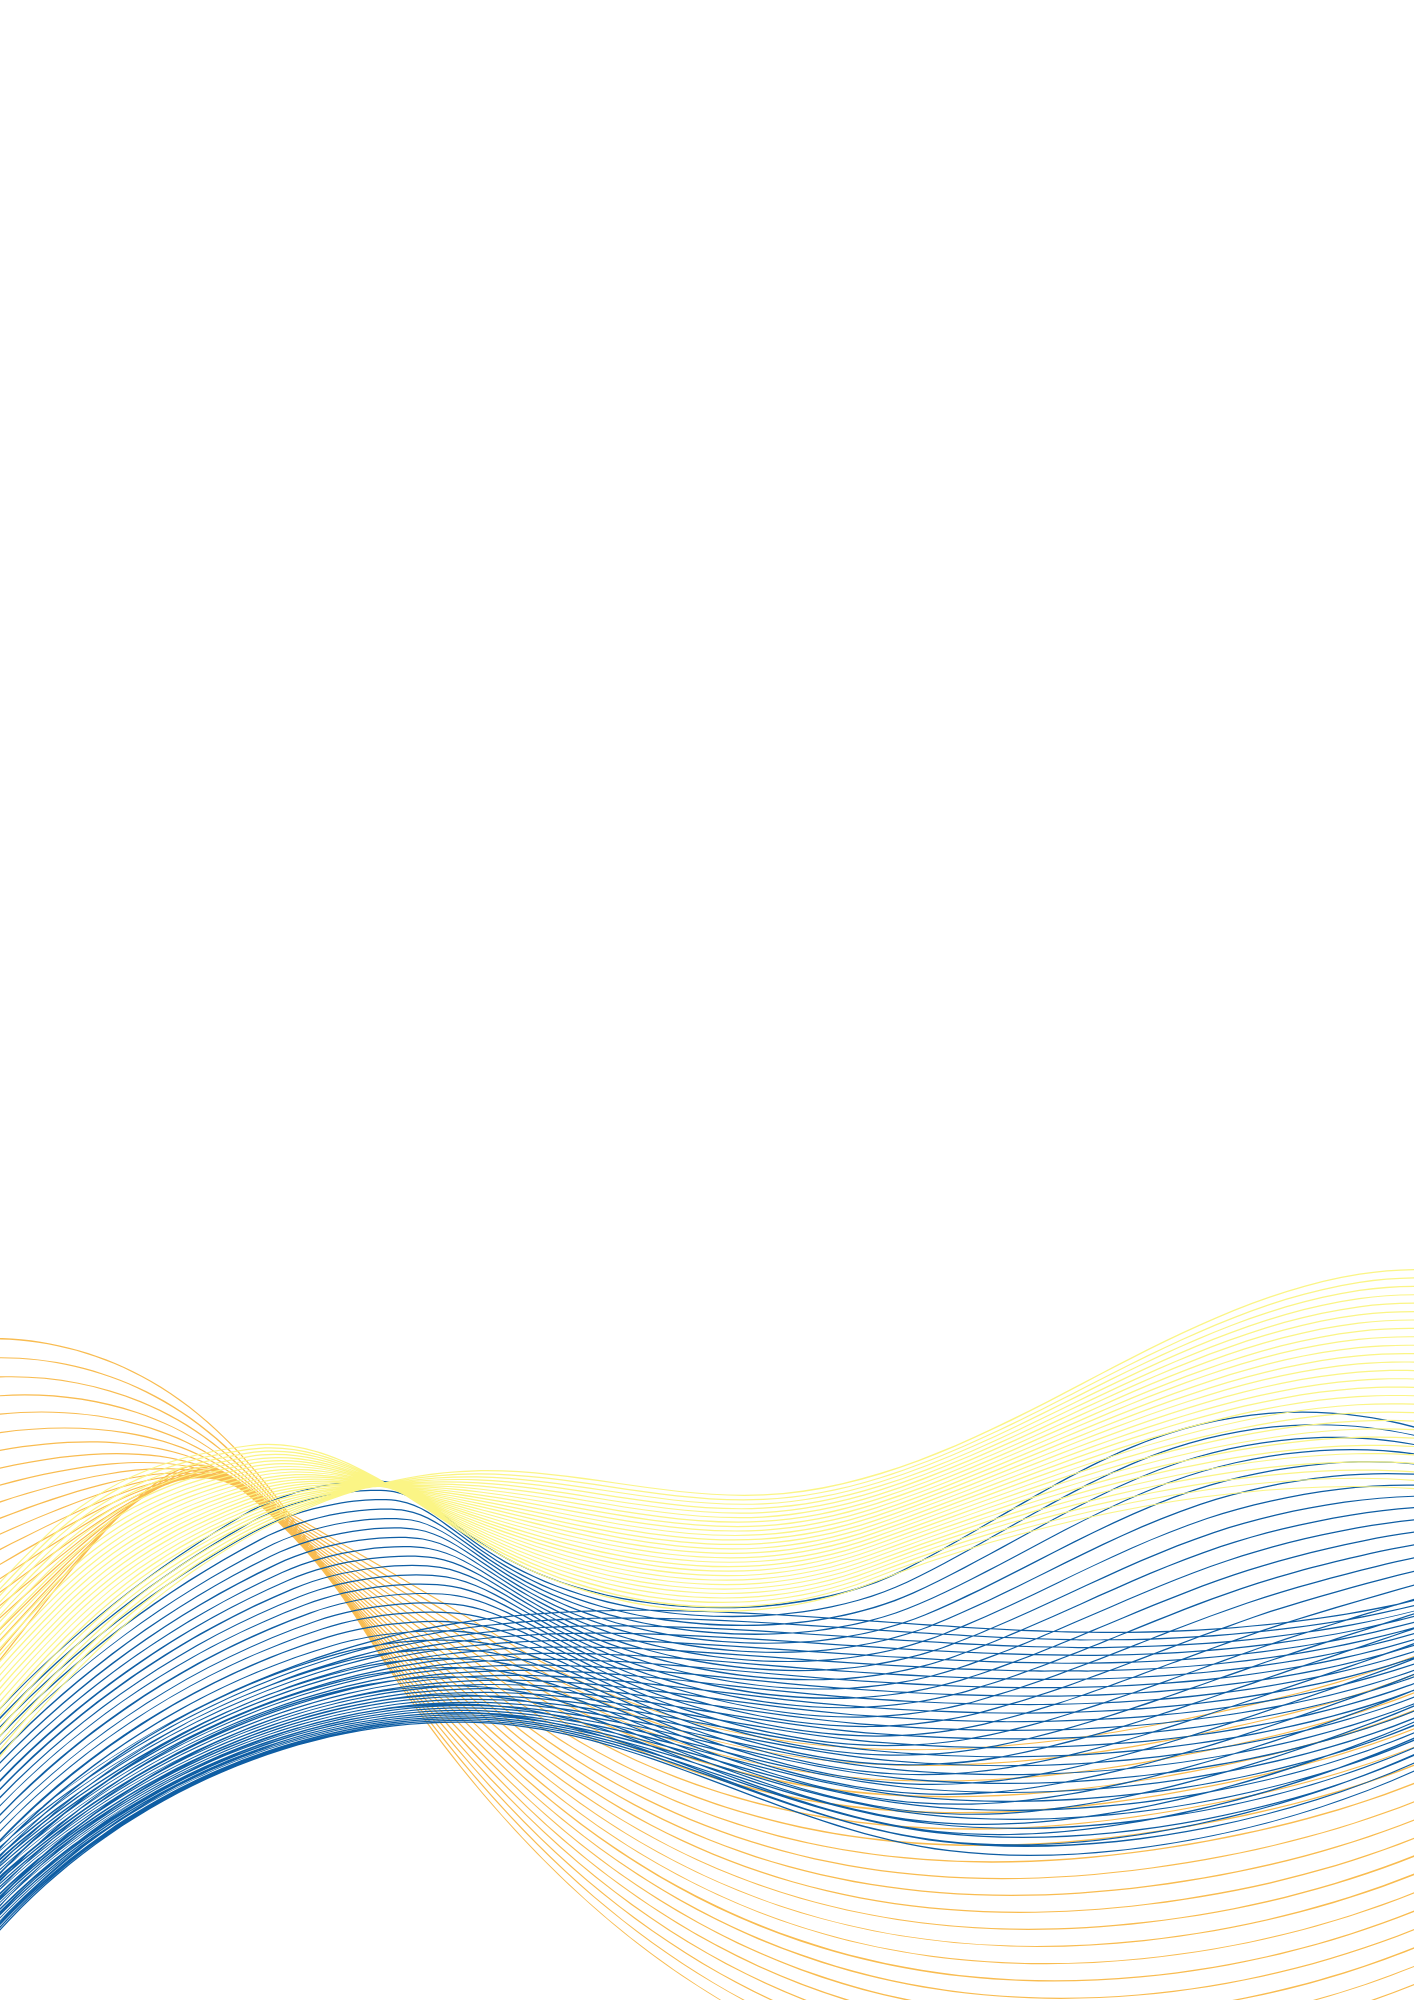
\includegraphics[width=\paperwidth]{../../shared/assets/media/image3.png}
 };

 % Preamble text overlay on bottom image
 \node[anchor=south west, inner sep=0pt] at ([xshift=1in, yshift=1.5cm]current page.south west) {
  \begin{minipage}{0.8\textwidth}
   \color{black}
   \textbf{Date de révision:} 20/11/2025 \\
   \textbf{Révisé par:} Conseil d'administration de la FCÉG
  \end{minipage}
 };
\end{tikzpicture}

\thispagestyle{empty}
\newpage


\newpage

% Setup headers/footers (after preamble so no header there)
\setupcfesheaders{Cahier des positions}

% Table of contents
\tableofcontents
\newpage

% Front matter
\section{La préambule}\label{la-preambule}

\subsection{La mission}\label{la-mission}

Un des principaux mandats de la Fédération canadienne étudiante de génie (FCEG) est de défendre les intérêts de plus de 80 000 étudiants en ingénierie répartis dans 45 établissements d'enseignement supérieur à travers le Canada. Au fil des ans, la FCEG a établi des partenariats avec des associations telles que le Bureau canadien d'accréditation des programmes de génie (BCAPG) et les Doyennes et doyens d'ingénierie Canada (DDIC), qui ont permis à la FCEG de défendre les intérêts des étudiants en génie, d'influencer la prise de décision concernant le programme d'études en génie et de façonner l'avenir de la profession d'ingénieur.

\subsection{Le portefeuille d'activités de plaidoyer de la FCEG, en bref}\label{le-portefeuille-dactivites-de-plaidoyer-de-la-fceg-en-bref}

Les activités de plaidoyer de la FCEG reposent sur deux (2) activités principales : les prises de position nationales et les enquêtes nationales. Les prises de positions sont destinées à être mises à jour régulièrement pour refléter les avancées et les reculs dans la défense des intérêts des étudiants en ingénierie et sont largement basées sur les données collectées dans le cadre des enquêtes nationales auprès des étudiants, qui sont censées être publiées une fois par an.

La FCEG a publié trois (3) enquêtes nationales à ce jour : l'édition de 2017, l'édition de 2020 portant sur des thèmes spécifiques à la COVID-19, et l'édition de 2023 sur le développement et le soutien des étudiants. La FCEG a adopté ses premières positions lors d'une assemblée générale à l'occasion de la Conférence canadienne sur le leadership en ingénierie (anciennement connu sous le nom de Congrès) en 2018, et elles ont depuis été mises à jour en 2024.

\subsection{Le cahier des positions}\label{le-cahier-des-positions}

Le cahier des positions récapitule les prises de positions officielles de la FCEG approuvées par ses membres, afin de mettre en avant les efforts des activités de plaidoyer dans divers aspects de l'expérience des étudiants en ingénierie. Le cahier des positions et les prises de position individuelles sont mis à la disposition des membres dans le cadre de leurs propres activités de plaidoyer. Ces documents s'inspirent des prises de position d'Ingénieurs Canada et constituent une ressource précieuse pour les membres, qui peuvent s'en inspirer pour leurs initiatives de plaidoyer institutionnelles.

\newpage

\section{La nomenclature}\label{la-nomenclature}

\begin{tblr}{colspec={lX}, rowsep=4pt}
  \textbf{AE/s}  & Association/s étudiante/s \\
  \textbf{ASSO}  & Association des étudiants en génie \\
  \textbf{BCAPG} & Bureau canadien d'accréditation des programmes de génie \\
  \textbf{CAÉGO} & Conseil des associations étudiantes en génie de l'Ontario \\
  \textbf{CD}    & Commissaire des données \\
  \textbf{CÉGA}  & Conseil d'étudiants de génie atlantique \\
  \textbf{CRÉIQ} & Confédération pour le rayonnement étudiant en ingénierie au Québec \\
  \textbf{DDIC}  & Doyennes et doyens d'ingénierie Canada \textit{(Note: anciennement connu sous CCDISA -- Conseil canadien des doyens d'ingénierie et des sciences appliquées)} \\
  \textbf{ECAIT} & Enseignement coopératif et apprentissage intégré au travail \\
  \textbf{FCEG}  & Fédération canadienne étudiante de génie \\
  \textbf{GdTES} & Groupe de travail sur les enjeux sociaux \\
  \textbf{GdTP}  & Groupe de travail plaidoyer \\
  \textbf{VPA}   & Vice-président académique \\
  \textbf{WESST} & L'équipe des sociétés étudiantes et génie de l'Ouest \\
\end{tblr}

\newpage


% Stances
\section{L'accréditation des ingénieurs}\label{laccreditation-des-ingenieurs}

\stanceinfo{\textbf{Congrès de la FCEG 2018} [2018-01-07]}{2024-01-02}

\officialstance{La Fédération canadienne étudiante de génie estime que le système d'accréditation des programmes d'ingénierie canadiens doit protéger les intérêt des étudiants en ingénierie en garantissant des normes élevées, cohérentes et réalisables pour la qualité de la formation en ingénierie, en faisant participer les étudiants au processus des visites d'accréditation et à l'élaboration des critères d'accréditation.}

\stanceheading{La position des étudiants}
\begin{itemize}
 \item Les étudiants sont une partie prenante essentielle de la formation des ingénieurs et devraient être activement consultés dans les discussions et les décisions relatives à l'accréditation des ingénieurs.
 \item Le processus de visite d'accréditation devrait être réformé pour mieux évaluer et intégrer les perspectives des étudiants tout au long de la visite.
 \item Un système d'accréditation efficace devrait être principalement axé sur les résultats de l'apprentissage, et toute mesure de la contribution des étudiants devrait être représentative du temps total d'apprentissage et ne pas favoriser l'apprentissage magistral par rapport à d'autres méthodes d'apprentissage.
 \item Les unités d'accréditation (UA) ne favorisent pas toujours les étudiants en ingénierie et n'affectent pas non plus la qualité de la formation d'ingénieur. Il conviendrait d'adopter une approche plus holistique, soit par le biais des UA, soit par une mesure différente de l'achèvement des attributs de l'ingénieur.
\end{itemize}

\stanceheading{Les recommandations aux partenaires, aux parties intéressées et aux autres entités}
\begin{itemize}
 \item La FCEG incite le BCAPG d'actualiser ses pratiques en matière de visites d'accréditation afin d'intégrer un retour d'information plus précieux et plus actif de la part des étudiants à la fin de chaque année d'accréditation.
 \item La FCEG incite le BCAPG à poursuivre ses efforts, notamment en ce qui concerne les Attributs des diplômés, afin de mieux refléter les résultats de l'apprentissage et le temps total d'apprentissage.
 \item La FCEG incite le BCAPG à réviser les Unités d'accréditation, car l'éducation et les concepts sont plus qu'un simple nombre quantifiable ou une case à cocher, car ils peuvent ne pas représenter avec précision la compréhension de l'étudiant.
 \item La FCEG incite le BCAPG à inclure les représentants des étudiants de la FCEG en tant que parties prenantes égales dans tous les projets, comités et groupes de travail liés à l'accréditation [réalisé].
 \item La FCEG incite les DDIC à collaborer sur des recommandations communes concernant le système d'accréditation actuel, basées sur les intérêts partagés des étudiants et des facultés.
 \item La FCEG incite les DDIC à avoir une communication transparente avec leurs écoles respectives afin que les voix des étudiants soient entendues au moment de la visite et que la meilleure formation d'ingénieur soit offerte.
 \item La FCEG incite le BCAPG à envisager d'intégrer davantage de possibilités d'expériences d'apprentissage extrascolaires dans le système d'accréditation actuel. Pour assurer la qualité de ces expériences d'apprentissage, la FCEG travaillera avec le BCAPG et les organismes provisoires de réglementation de l'ingénierie afin de créer un cadre et un ensemble de normes rigoureux.
 \item La FCEG incite le BCAPG de standardiser et de réguler la qualité des stages offerts par les programmes universitaires en ingénierie au Canada
 \item La FCEG incite les DDIC à régulièrement mettre à jour ses offres de cours et ses politiques pour les adapter à l'évolution des critères des Unités d'accréditation et aux améliorations apportées durant chaque année universitaire.
\end{itemize}

\stanceheading{Ce que fait la FCEG}
\begin{itemize}
 \item La FCEG assure la représentation des étudiants en tant qu'observateurs au sein du BCAPG depuis plusieurs années. En 2015, la responsabilité de plaidoyer auprès du BCAPG a été formalisée.
 \item La FCEF a assisté à une rencontre des DDIC pour la première fois en 2017, et a discuté d'une collaboration à venir sur des enjeux liés à l'accréditation.
 \item Le réunions du BCAPG accordent à la FCEG le droit de s'exprimer lors des sessions ouvertes, tel que décrit dans la \href{https://engineerscanada.ca/sites/default/files/2022-02/Board-Policy-Manual-Combined-e.pdf}{politique} ci-dessous [1]:
 \begin{itemize}
  \item 6.9.1 F.1 Observateurs présents lors des réunions (1) Le BCAPG doit inviter à ses réunions, à titre d'observateurs, les représentants suivants qui se verront accorder le droit de parole pendant les séances ouvertes : a) Le président ou la présidente de la Fédération Canadienne des Étudiant(e)s en génie (FCEG) ou son mandataire;
  \item De plus, la Politique 7.2 du Conseil d'Administration d'Ingénieurs Canada demande au BCAPG d'entretenir des relations avec la FCEG:
  \begin{itemize}
   \item Les étudiants en génie sont des parties prenantes importantes de l'agrément. En plus de solliciter la rétroaction des étudiants lors des visites d'évaluation de programmes, le Bureau d'agrément est tenu de maintenir des liens avec la FCEG et d'inviter un représentant à observer ses réunions et à lui soumettre un rapport. Tous les frais de déplacement de ce représentant sont assumés par Ingénieurs Canada.
  \end{itemize}
 \end{itemize}
 \item Le BCAPG a mis à jour son modèle de programme de visite d'accréditation basé sur les commentaires des parties prenantes, y compris la FCEG, en prévoyant plus de temps pour la participation des étudiants pendant les visites d'accréditation.
 \item La FCEG a inclus une section sur les programmes d'ingénierie dans l'enquête nationale de 2023 afin d'évaluer la connaissance générale du BCAPG ainsi que la compréhension et l'inclusion des Unités d'accréditation.
 \item Le BCAPG a été consulté pour les questions de l'enquête nationale de 2023 et pour la mise à jour de la documentation sur le cahier de positions.
\end{itemize}

\stanceheading{Ce que la FCEG envisage de faire}
\begin{itemize}
 \item La FCEG s'efforcera d'être incluse dans tous les projets et comités pertinents liés au BCAPG.
 \item La FCEG créera et distribuera en permanence une enquête nationale afin d'actualiser ses connaissances sur les expériences des étudiants en matière d'accréditation et de services fondés sur l'accréditation. Les questions de l'enquête seront consultées chaque année par le BCAPG afin d'éviter tout recoupement avec leur propre enquête.
 \item La FCEG actualisera sa position sur l'accréditation au fur et à mesure que des changements significatifs interviendront dans la politique et la réglementation.
 \item La FCEG demandera aux DDIC de rendre compte des changements non suivis au sein de leurs universités en ce qui concerne les nouvelles politiques et réglementations spécifiques aux attributs de l'ingénierie.
 \item La FCEG recueillera des commentaires supplémentaires spécifiquement liés aux visites d'accréditation afin d'examiner le point de vue des étudiants sur la qualité des visites d'accréditation qui ont eu lieu.
\end{itemize}

\newpage

\section{Les cours facultatifs de langues}\label{les-cours-facultatifs-de-langues}

\stanceinfo{\textbf{Congrès de la FCEG 2018} [2018-01-07]}{2024-01-02}

\officialstance{La Fédération canadienne étudiante de génie croit que les étudiants canadiens en génie devraient avoir l'occasion de suivre des cours facultatifs de langue dans le cadre de leur programme de premier cycle afin d'enrichir leur diplôme d'ingénierie.}

\stanceheading{La position des étudiants}
\begin{itemize}
 \item En 2018, le BCAPG a mis à jour ses \href{https://engineerscanada.ca/sites/default/files/accreditation/2021-2022-cycle/accreditation-criteria-procedures-2020.pdf}{critères et procédures d'accréditation} [2] afin d'accepter explicitement les cours facultatifs de langue dans le cadre de leurs exigences en matière « d'études complémentaires » pour les programmes d'ingénierie au Canada ; cependant, environ 23\% des écoles d'ingénieurs accréditées au Canada n'ont pas encore reflété cette évolution au sein de leurs facultés.
 \item En 2022, le critère a été supprimé 3.4.5.2 comme indiqué ci-dessous, où la FCEG a constaté qu'il reste inscrit sur certains sites d'universités d'études complémentaires :
 \begin{itemize}
  \item [Supprimé] Critère 3.4.5.2 L'enseignement des langues peut être inclus dans les études complémentaires à condition qu'il ne soit pas suivi pour remplir une condition d'admission. En outre, le contenu du programme d'études qui transmet principalement des compétences linguistiques peut être pris en compte dans l'unité d'accréditation (UA) requise pour les études complémentaires, mais ne peut pas être utilisé pour satisfaire aux exigences relatives aux matières qui traitent des questions centrales, des méthodologies et des processus de pensée des sciences humaines et sociales.
  \item Le FCEG est en accord avec la déclaration supprimée, car même les matières qui traitent d'autres langues sont inclusives pour l'enrichissement des étudiants en ingénierie en dehors de leurs cours techniques.
 \end{itemize}
 \item La connaissance d'une autre langue et des matières connexes est un atout précieux pour l'avenir d'un étudiant en ingénierie et les étudiants doivent disposer d'un éventail complet et approprié d'options linguistiques.
\end{itemize}

\stanceheading{Les recommandations aux partenaires, aux parties intéressées et aux autres entités}
\begin{itemize}
 \item La FCEG incite le BCAPG à aider les 23 \% d'établissements canadiens restants à interpréter leur politique actuelle sur les cours facultatifs en publiant une déclaration interprétative officielle sur le sujet, énonçant des critères supplémentaires.
 \item La FCEG incite les DDIC à encourager ses facultés membres à revoir et à reconsidérer leurs offres de cours facultatifs, et à permettre aux étudiants en ingénierie de s'inscrire à des cours de langue qui comptent pour l'obtention de leur diplôme, en plus et y compris des deux langues officielles du Canada.
 \item La FCEG incite les DDIC à mettre à jour ses politiques et ses informations disponibles sur ses calendriers académiques afin de suivre et de décrire avec précision les politiques et procédures du BCAPG concernant ce qui est considéré comme un cours facultatif.
 \item La FCEG incite les associations des étudiants en génie à soutenir les efforts de plaidoyer nationaux et à tirer parti de la mise à jour de la politique du BCAPG pour défendre la mise en œuvre de cours facultatifs de langue dans leur programme afin de profiter des avantages du multilinguisme dans un pays diversifié et un monde de plus en plus globalisé.
 \item La FCEG incite ses membres à remettre en question le cursus actuellement en place, et à poursuivre des études qui les inspirent en langues et qui enrichissent leur formation d'ingénieur, même si des autorisations supplémentaires sont nécessaires pour les poursuivre.
\end{itemize}

\stanceheading{Ce que fait la FCEG}
\begin{itemize}
 \item Les discussions de la FCEG sur l'interprétation de la politique des cours facultatifs de langues sur deux périodes de mandat ont été acceptées par le Comité des politiques et procédures du BCAPG qui a accepté que les sections linguistiques soient considérées comme des cours à option ouverts avant la Réunion du Président (RdP) de 2019.
 \item La FCEG a créé et continue de mettre à jour un dossier de plaidoyer pour aider les étudiants à plaider en faveur des cours facultatifs de langues au niveau de l'établissement.
 \item La FCEG a examiné les options linguistiques au sein des universités d'ingénierie accréditées au Canada et a dressé une liste des universités qui ne respectent pas la politique actuelle.
 \item La FCEG a présenté des données sur les universités BCAPG qui ne respectent pas la politique actuelle ou qui utilisent des informations obsolètes afin de faciliter le dialogue entre les DDIC et le BCAPG.
\end{itemize}

\stanceheading{Ce que la FCEG envisage de faire}
\begin{itemize}
 \item La FCEG fournira des ressources sur les cours facultatifs de langues afin de fournir à ses écoles membres les informations dont elles ont besoin pour plaidoyer en faveur de la modification des cours facultatifs dans leurs établissements respectifs.
 \item La FCEG fournira une analyse des avantages des cours facultatifs de langues disponibles comme études complémentaires et de la manière dont ils enrichissent la formation en ingénierie.
 \item La FCEG travaillera avec les DDIC pour lui faire connaître les politiques et les documents qui ne correspondent pas à la politique et aux procédures actuelles du BCAPG ou qui ne sont pas tout à fait exacts.
 \item La FCEG poursuivra ses efforts de plaidoyer et continuera la discussion sur l'importance du bilinguisme/multilinguisme lors des présentations des partenaires externes sur l'avenir de la formation des ingénieurs.
\end{itemize}

\newpage

\section{La santé mentale et la charge de travail des étudiants}\label{la-sante-mentale-et-la-charge-de-travail-des-etudiants}

\stanceinfo{\textbf{Congrès de la FCEG 2018} [2018-01-07]}{2024-01-02}

\officialstance{La Fédération canadienne étudiante de génie estime que les étudiants en ingénierie sont confrontés à des problèmes de santé mentale en raison de la structure et de la charge de travail de leurs programmes. Toutes les parties prenantes, y compris le corps enseignant, les organismes d'accréditation et les leaders étudiants, ont la responsabilité de revoir et de modifier leurs pratiques afin d'offrir aux étudiants un environnement d'apprentissage sain et efficace.}

\stanceheading{La position des étudiants}
\begin{itemize}
 \item Les étudiants en ingénierie présentent un risque élevé d'effets négatifs sur la santé mentale, avec quatre thèmes récurrents présents en littérature [3];
 \begin{itemize}
  \item La charge de travail des ingénieurs est un facteur de stress déterminant;
  \item Il existe des obstacles qui empêchent les étudiants en ingénierie de chercher de l'aide pour des problèmes de santé mentale;
  \item Les pairs s'appuient davantage les uns sur les autres pour faire face au stress et aux problèmes de santé mentale;
  \item La pandémie de COVID-19 a exacerbé les problèmes de santé mentale des étudiants.
 \end{itemize}
 \item Les étudiants en ingénierie se déclarent très stressés, anxieux et dépressifs, certains documents faisant état de 28 \% de stress modéré à extrêmement grave, de 35 \% d'anxiété modérée à extrêmement grave et de 34 \% de dépression modérée à extrêmement grave, d'après une enquête réalisée en 2021 [4].
 \item La perception généralisée selon laquelle un niveau de stress élevé et une mauvaise santé mentale sont normaux et prévisibles dans le domaine de l'ingénierie est préjudiciable et ne tient pas compte des problèmes de santé mentale des étudiants de premier cycle actuels et de ceux qui veulent choisir l'ingénierie.
 \item La charge de travail excessive des étudiants est probablement l'une des principales causes de ces effets négatifs sur la santé mentale, et des mesures devraient être prises pour réduire le stress universitaire lié à la charge de travail.
 \item Les problèmes de santé mentale touchent de manière disproportionnée les femmes et les autres minorités, notamment les personnes LGBTQ2S+, les autochtones et les personnes de couleur [4].
 \item Les étudiants en ingénierie sont peu enclins à rechercher un soutien en matière de santé mentale, même s'ils déclarent eux-mêmes des niveaux plus élevés de détresse en matière de santé mentale, en raison de différents facteurs, notamment physiques et culturels [5].
\end{itemize}

\stanceheading{Les recommandations aux partenaires, aux parties intéressées et aux autres entités}
\begin{itemize}
 \item La FCEG demande au BCAPG d'étudier la possibilité de modifier les critères d'accréditation afin de mieux tenir compte de la charge de travail des étudiants et d'exiger l'accès à des services de santé mentale de base pour tous les étudiants de premier cycle en ingénierie.
 \item La FCEG incite le BCAPG à étudier et à revoir les unités d'accréditation (UA) avec leurs heures respectives afin de s'assurer qu'elles restent réalisables dans le cadre d'une charge de travail complète pour les étudiants.
 \item La FCEG incite les DDIC à examiner la Norme nationale pour la santé mentale et le bien-être pour les étudiants du postsecondaire de la Commission de la santé mentale du Canada (Normes postsecondaires de la CSMC) [6] et à mettre en œuvre ces normes dans leurs facultés d'ingénierie.
 \item La FCEG incite le BCAPG à tenir ses instructeurs responsables de veiller à ce que la charge de travail ne nuise pas aux étudiants en ingénierie et à s'efforcer de mettre en place davantage de possibilités d'apprentissage tout au long de la vie, de possibilités d'apprentissage basées sur les problèmes et moins de défis académiques à fort enjeu.
 \item La FCEG incite Ingénieurs Canada et les DDIC de s'associer à la FCEG pour faire de la recherche liée à la santé mentale et à la charge de travail des étudiants dans le but de clarifier les impacts de la charge de travail sur la santé mentale des étudiants en ingénierie et les meilleures procédures pour l'améliorer.
 \item La FCEG incite ses organisations régionales partenaires (WESST, CAÉGO, CRÉIQ, CÉGA) à collaborer à des initiatives futures en matière de charge de travail et de santé mentale des étudiants, ce qui pourrait inclure un système de suivi de la charge de travail ou une deuxième enquête nationale auprès des étudiants.
 \item La FCEG incite ses membres à évaluer objectivement leur charge de travail et à trouver des lacunes ou des problèmes dans le cursus d'ingénierie de leurs écoles, et à soulever la question auprès de leurs organisations régionales.
\end{itemize}

\stanceheading{Ce que fait la FCEG}
\begin{itemize}
 \item La FCEG a mené une enquête nationale auprès des étudiants en 2023 afin de recueillir des données sur la santé mentale des étudiants en génie ainsi que sur la charge de travail et la perception des étudiants. La FCEG a organisé des séances et des conférences sur la santé mentale des étudiants, en mettant en évidence les initiatives étudiantes et l'épuisement des étudiants bénévoles, lors de ses principaux événements, notamment la Conférence canadienne sur le leadership en ingénierie (CCLI) et la Conférence sur la diversité en ingénierie (CDI).
 \item La FCEG a créé un répertoire des meilleures pratiques en matière de santé mentale disponible à toute organisation membre via le dossier \textit{Google Drive} externe.
\end{itemize}

\stanceheading{Ce que la FCEG envisage de faire}
\begin{itemize}
 \item La FCEG continuera à faciliter le partage des meilleures pratiques en matière de santé mentale entre ses sociétés membres et à mettre à jour les ressources pour la défense de la santé mentale des étudiants, le cas échéant.
 \item La FCEG poursuivra ses recherches sur les conséquences spécifiques d'une mauvaise santé mentale des étudiants et sur les meilleures pratiques pour améliorer la santé mentale dans les écoles d'ingénieurs.
 \item Le FCEG évaluera comment il peut mieux promouvoir la santé mentale des étudiants en interne par le biais des opérations et du contenu de ses événements.
 \item La FCEG assurera le suivi avec les parties prenantes concernées, y compris les DDIC, afin de garantir un examen systématique et régulier de la charge de travail et des horaires des programmes d'ingénierie, ainsi que des politiques mises en place pour protéger les étudiants.
 \item La FCEG examinera et appliquera les Normes Postsecondaires de la CSMC à la planification des conférences, à la motivation pour la défense des intérêts et aux pratiques de l'équipe interne.
\end{itemize}

\newpage

\section{La qualité des stages en ingénierie}\label{la-qualite-des-stages-en-ingenierie}

\stanceinfo{\textbf{Congrès de la FCEG 2018} [2018-01-07]}{2024-01-02}

\officialstance{La Fédération canadienne étudiante de génie estime que la qualité des programmes de stages en ingénierie au Canada est inégale et souvent inférieure aux normes, et que les programmes d'ingénierie ont la responsabilité de revoir leurs pratiques afin d'offrir aux étudiants un meilleur rapport qualité-prix pour leurs frais de programme.}

\stanceheading{La position des étudiants}
\begin{itemize}
 \item La satisfaction des étudiants à l'égard de la qualité des programmes de stages est faible dans l'ensemble du Canada, ce qui traduit une insatisfaction générale à l'égard de la valeur des services de stages offerts par les écoles d'ingénieurs, notamment en ce qui a trait aux possibilités, aux ressources fournies et à l'accessibilité.
 \item L'absence de réglementation des programmes de stages en génie entraîne une plus grande variation et des normes moins élevées pour les services offerts aux étudiants, comparativement à d'autres domaines de la formation en génie.
 \item Les lacunes des programmes de stages varient considérablement d'un établissement à l'autre, ce qui signifie qu'une réponse efficace aux problèmes liés aux programmes de stages doit être apportée à l'échelle locale.
\end{itemize}

\stanceheading{Les recommandations aux partenaires, aux parties intéressées et aux autres entités}
\begin{itemize}
 \item La satisfaction des étudiants à l'égard de la qualité des programmes de stages est faible dans l'ensemble du Canada, ce qui traduit une insatisfaction générale à l'égard de la valeur des services de stages offerts par les écoles d'ingénieurs, notamment en ce qui a trait aux possibilités, aux ressources fournies et à l'accessibilité.
 \item L'absence de réglementation des programmes de stages en génie entraîne une plus grande variation et des normes moins élevées pour les services offerts aux étudiants, comparativement à d'autres domaines de la formation en génie.
 \item Les lacunes des programmes de stages varient considérablement d'un établissement à l'autre, ce qui signifie qu'une réponse efficace aux problèmes liés aux programmes de stages doit être apportée à l'échelle locale.
\end{itemize}

\stanceheading{Ce que fait la FCEG}
\begin{itemize}
 \item La FCEG a fait de la qualité des stages un domaine d'intérêt pour son Enquête nationale des étudiants de 2017 et ses recherches connexes, afin de déterminer l'ampleur des problèmes liés aux programmes de stages dans l'ensemble du Canada.
 \item La FCEG a inclus des questions sur les stages et le développement professionnel dans l'enquête nationale de 2023 afin de déterminer les exigences relatives aux stages et les ressources disponibles dans les établissements.
\end{itemize}

\stanceheading{Ce que la FCEG envisage de faire}
\begin{itemize}
 \item La FCEG travaillera avec ses partenaires pour créer des ressources afin de partager des informations de base sur les pratiques des programmes d'ingénierie à travers le Canada, et pour plaider auprès des facultés en faveur de changements efficaces.
 \item La FCEG étudiera les mérites d'un plaidoyer auprès de l'Enseignement coopératif et l'apprentissage en milieu de travail Canada pour améliorer leur agrément des programmes de stages en ingénierie.
 \item La FCEG rapportera aux DDIC les données recueillies dans le cadre de l'enquête nationale sur les stages, afin de fournir une orientation à leurs programmes individuels.
 \item La FCEG travaillera avec les organisations régionales (WESST, CAÉGO, CRÉIQ, CÉGA) afin d'obtenir de l'information au niveau régional sur les pratiques et les politiques communes en matière de stages en génie.
\end{itemize}

\newpage

\section{Le développement durable}\label{le-developpement-durable}

\stanceinfo{\textbf{Congrès de la FCEG 2018} [2018-01-07]}{2024-01-02}

\officialstance{La Fédération canadienne étudiante de génie estime que le développement durable est une considération essentielle dans la pratique de l'ingénierie et qu'il est nécessaire d'éduquer et d'impliquer ses membres sur les questions de développement durable, tout en évaluant et en améliorant le programme d'études sur le développement durable dans le domaine de l'ingénierie.}

\stanceheading{La position des étudiants}
\begin{itemize}
 \item Les ingénieurs ont la responsabilité de faire primer la sécurité, la santé et le bien-être du public et de tenir compte de l'environnement, ce qui implique la responsabilité d'effectuer un travail durable pour les générations futures.
 \item Les futures générations d'ingénieurs devraient recevoir une formation approfondie et s'investir dans les pratiques de développement durable de l'ingénierie avant l'obtention de leur diplôme, par le biais d'applications appropriées dans le cadre du programme d'études d'ingénierie.
 \item La FCEG devrait évaluer la durabilité de ses opérations afin de réformer et d'améliorer ses pratiques si nécessaire.
 \item Le travail de plaidoyer autour de la durabilité doit être évalué dans l'optique des étudiants en ingénierie, des opportunités d'emploi et de l'avenir de l'ingénierie.
\end{itemize}

\stanceheading{Les recommandations aux partenaires, aux parties intéressées et aux autres entités}
\begin{itemize}
 \item La FCEG incite le BCAPG à intégrer des unités d'accréditation axées sur le développement durable dans tous les diplômes d'ingénierie, et à garantir que l'ensemble des étudiants en ingénierie diplômés possèdent ces compétences.
 \item La FCEG encourage ses membres à plaider en faveur de l'importance du développement durable dans leurs activités quotidiennes au sein de leur propre institution, tout en les incitant à participer aux conférences respectives de la FCEG. Cela inclut la promotion de l'idée d'un désinvestissement institutionnel et la fourniture de ressources dédiées au développement durable.
 \item La FCEG encourage les DDIC à soutenir les initiatives, les équipes et les pratiques de développement durable au sein de leurs institutions respectives. Elle les incite également à établir des partenariats avec des organisations en vue de créer un campus d'ingénierie plus durable.
\end{itemize}

\stanceheading{Ce que fait la FCEG}
\begin{itemize}
 \item La FCEG organise chaque année une conférence nationale sur le développement durable en ingénierie dans l'une de ses écoles membres, dans le but d'éduquer et d'engager directement les étudiants en ingénierie sur les pratiques durables liées à la profession, qu'ils pourront rapporter et mettre en œuvre des idées dans leurs universités.
 \item La FCEG continuera à mettre à jour les meilleures pratiques en matière de développement durable pour son usage et celui de ses sociétés membres, y compris La Banque des meilleures pratiques en matière de développement durable, ainsi que d'autres ressources d'apprentissage utiles liées au développement durable.
\end{itemize}

\stanceheading{Ce que la FCEG envisage de faire}
\begin{itemize}
 \item La FCEG effectuera une analyse annuelle de l'empreinte environnementale de ses activités et réformera ses activités pour les aligner sur les pratiques durables dans la mesure du possible.
 \item La FCEG contribuera à l'élaboration d'une documentation sur les lignes directrices de la conférence en matière de développement durable, afin de prendre en compte les pratiques durables dans les processus de planification et d'exécution. En tant qu'organisation nationale d'étudiants, la FCEG a un rôle majeur à jouer pour ouvrir la voie à des actions durables en tant qu'organisation et pour motiver ensuite les écoles membres.
 \item La FCEG peut élaborer des documents d'orientation pour elle-même et ses organisations membres afin de réduire leur impact sur l'environnement, par le biais d'un document évolutif décrivant les meilleures pratiques. Ce document sera revu et mis à jour chaque année afin de refléter tout changement dans les meilleures pratiques.
\end{itemize}

\newpage

\section{L'équité, la diversité et l'inclusion}\label{lequite-la-diversite-et-linclusion}

\stanceinfo{\textbf{Congrès de la FCEG 2019} [2019-01-04]}{2024-01-02}

\officialstance{La Fédération canadienne étudiante de génie (FCEG) estime que l'équité, la diversité et l'inclusion (EDI) sont essentielles à la durabilité de la profession d'ingénierie et à sa contribution à l'intérêt public. L'inclusion et la participation accrue des groupes sous-représentés apportent des perspectives et des expériences différentes qui aident les ingénieurs à résoudre les problèmes au sein de la profession d'ingénieur et dans les programmes d'études de premier cycle.}

\stanceheading{La position des étudiants}
\begin{itemize}
 \item Le renforcement de la diversité et de la représentation des groupes minoritaires au sein de l'ingénierie permet de relever les défis et de créer des solutions aux problèmes d'ingénierie qui profitent à tous.
 \item Les étudiants en ingénierie doivent avoir accès à l'égalité des chances dans le domaine de l'ingénierie, indépendamment de leur âge, de leur origine ethnique, de leur race, de leur sexe, de leur orientation sexuelle, de leur situation économique, de leur capacité, de leur religion ou d'autres origines diverses. Ces possibilités comprennent l'accès aux ressources et aux possibilités qui favorisent leur développement en tant qu'ingénieur (stages, conférences sur l'ingénierie, etc.).
 \item L'augmentation de la diversité des étudiants dans les programmes d'ingénierie permet d'améliorer la formation des ingénieurs en exposant les étudiants à davantage de perspectives, d'expériences et de manières de penser.
 \item La diversité sera favorisée à un taux plus élevé et plus efficace dans un environnement inclusif en contribuant à la rétention des groupes sous-représentés. Afin de créer un environnement inclusif, il convient de mettre en place une éducation et des initiatives autour des thèmes de la diversité afin d'éduquer les individus à améliorer l'accessibilité pour les personnes diverses et à réduire les préjugés inconscients.
 \item L'intégration des populations autochtones dans l'ingénierie est un sujet important, mais peu discuté, étant donné que le Canada se trouve sur des terres autochtones traditionnelles et non cédées et que son existence est le résultat d'une colonisation dont les effets sont encore présents aujourd'hui.
 \item La FCEG approuve également les Énoncés de principe nationaux d'Ingénieurs Canada et l'initiative 30 en 30 d'Ingénieurs Canada, qui vise à accroître la proportion des personnes s'identifiant en tant qu'ingénieurs nouvellement agréés à 30 pour cent d'ici 2030.
 \item Les groupes sous-représentés sont souvent désavantagés en matière d'accès à l'ingénierie, d'accessibilité et de capacité à prospérer en raison d'obstacles systémiques qui les affectent de manière disproportionnée.
 \item Créer un environnement inclusif au sein de l'ingénierie implique l'établissement d'un cadre, d'une culture et de pratiques sécurisés qui accueillent et respectent les contributions des individus issus de milieux, d'expériences et de perspectives divers.
\end{itemize}

\stanceheading{Les recommandations aux partenaires, aux parties intéressées et aux autres entités}
\begin{itemize}
 \item La FCEG demande au Réseau 30 en 30 d'Ingénieurs Canada d'étudier les raisons pour lesquelles les taux de rétention des femmes sont faibles dans les études de premier cycle et de les présenter officiellement à d'autres parties prenantes, y compris au conseil d'administration d'Ingénieurs Canada.
 \item La FCEG demande au Réseau 30 en 30 d'Ingénieurs Canada de commencer à élaborer des plans secondaires si le programme 30 en 30 n'est pas réalisé à l'échelle du Canada, et d'intégrer les voix des étudiants dans la nouvelle proposition.
 \item La FCEG demande aux DDIC de continuer à promouvoir le recrutement d'identités diverses parmi les nouveaux étudiants en génie au moyen d'initiatives qui favorisent l'équité au sein de la communauté des ingénieurs. (i.e. bourses d'études pour les communautés sous-représentées)
 \item La FCEG demande au BCAPG d'intégrer l'équité, la diversité et l'inclusion (ÉDI) dans les attributs des diplômés, de façon similaire à l'impact du génie sur la société et l'environnement, de décrire l'importance de la formation en ÉDI et de toujours s'assurer que les considérations liées à l'ÉDI sont prises en compte dans la profession de génie.
 \item La FCEG demande aux DDIC d'intégrer une vice-doyenne à l'équité, à la diversité et à l'inclusion ou un poste de rang similaire au sein de leur établissement afin d'assurer une accessibilité équitable, diversifiée et inclusive au génie et d'offrir un soutien aux groupes sous-représentés.
 \item La FCEG demande aux DDIC d'offrir une formation sur l'équité, la diversité et l'inclusion à leurs instructeurs et à leurs étudiants, en particulier aux étudiants qui représentent l'ensemble de l'établissement.
 \item La FCEG demande aux administrateurs des établissements, avec le soutien des doyens des facultés d'ingénierie du Canada, de mettre en œuvre et d'appliquer des protocoles pour traiter les cas de discrimination et de harcèlement au sein de la communauté des ingénieurs.
 \item La FCEG incite le BCAPG et les DDIC à promouvoir les principes de gestion dans les programmes d'études, afin que les étudiants soient mieux équipés pour prendre en compte et défendre les valeurs de l'ÉDI sur leur lieu de travail à la fin de leurs études.
 \item Enfin, la FCEG incite nos membres à examiner les traditions d'ingénierie qu'ils défendent et à considérer avec un regard critique si elles respectent et contribuent à créer un environnement inclusif pour tous. En outre, la FCEG incite ses membres à rechercher des occasions de promouvoir la connaissance d'ÉDI parmi les étudiants et à créer des initiatives qui soutiennent l'équité, la diversité et l'inclusion au sein de leurs institutions.
\end{itemize}

\stanceheading{Ce que la FCEG envisage de faire}

La FCEG prévoit de renforcer son soutien et sa promotion de l'inclusion au sein de la communauté des étudiants en ingénierie en fournissant des ressources et en partageant les meilleures pratiques avec les écoles membres en ce qui concerne l'organisation d'événements inclusifs et la mise en place d'orientations/de formations sur l'inclusion au sein de leurs communautés respectives.

\begin{itemize}
 \item Poursuivre ses efforts en matière d'inclusion en proposant des orientations sur l'inclusion lors de tous les événements, ainsi qu'en approfondissant l'évaluation des risques en matière d'inclusion lors des événements;
 \item Explorer de nouveaux partenariats avec des organisations axées sur la diversité et l'inclusion (Catalyst Canada, Actua, Women in Engineering, Association canadienne pour la santé mentale, National Society of Black Engineers, Laboratoire d'innovation en ingénierie, etc.);
 \item Donner la priorité à l'intégration active du bilinguisme dans toutes les activités de la FCEG, ainsi qu'au cœur de l'organisation;
 \item Élaborer des lignes directrices pour la planification d'événements inclusifs spécifiques aux activités de la FCEG afin d'aider à identifier, supprimer et prévenir les obstacles susceptibles d'empêcher quiconque de participer pleinement aux activités de la FCEG, et veiller à ce que ces considérations soient prises en compte dès les premières étapes de la planification de chaque activité;
 \item Respecter tous les engagements énoncés dans la Charte des champions afin d'appuyer officiellement l'initiative 30 en 30 d'Ingénieurs Canada, notamment en désignant chaque année, lors de la réunion de printemps, un champion qui participe au groupe des champions et qui s'engage activement dans le réseau 30 en 30;
 \item Mettre en pratique le formulaire de signalement des cas d'exclusion et des actes préjudiciables, qui permet aux membres de faire part de leurs commentaires;
 \item Donner la priorité aux événements et activités sans barrières lors des conférences de la FCEG, en proposant des alternatives lorsque cela n'est pas possible;
 \item Créer une boîte à outils pour les membres de la FCEG sur l'équité, la diversité et l'inclusion à l'intention des membres, qui comprendra notamment les éléments suivants :
 \begin{itemize}
  \item La formation sur l'équité, la diversité et l'inclusion
  \item Le programme de certification ÉDI
  \item Les pratiques exemplaires pour les organisations externes
  \item Les statistiques démographiques canadiennes sur le génie
  \item L'accès aux partenaires de la FCEG pour la défense des intérêts locaux
  \item Les mécanismes de retour d'information
 \end{itemize}
\end{itemize}

\newpage

\section{La cérémonie du jonc}\label{la-ceremonie-du-jonc}

\stanceinfo{\textbf{CESS de la FCÉG 2023} [2023-03-02]}{2024-01-02}

\officialstance{La Fédération canadienne étudiante de génie estime que la cérémonie du jonc est une cérémonie de transition nécessaire pour les étudiants en génie, mais que, dans son état actuel, elle est obsolète et ne représente plus pleinement l'ingénierie de l'ère moderne. Elle limite plutôt la description de la profession d'ingénieur et possède un ton d'exclusion, et elle devrait être modifiée pour reconnaître l'obligation de tous les ingénieurs.}

\stanceheading{La position des étudiants}
\begin{itemize}
 \item La cérémonie du jonc est un rite de passage essentiel pour les étudiants en ingénierie. Elle est très appréciée des diplômés après l'obtention d'un diplôme long et difficile.
 \item Dans le meilleur des cas, la cérémonie du jonc peut contribuer à un sentiment d'appartenance et de communauté dans le domaine de l'ingénierie.
 \item Le rituel original ne s'adresse pas à tous les étudiants en ingénierie, ce qui les déçoit. Le rituel restreint la pratique de l'ingénierie en dehors des formes de travail originales lorsque le rituel a été promulgué pour la première fois et présente une vision du monde dépassée en ce qui concerne le colonialisme, le racisme et le sexisme.
 \item Chaque camp organise sa propre cérémonie avec peu de surveillance de la part de la corporation des sept gardiens.
 \item Tous les étudiants en ingénierie devraient se sentir inclus, à l'aise et respectés pendant le Rituel de l'appel de l'ingénieur.
\end{itemize}

\stanceheading{L'enjeu}

La Cérémonie du jonc est l'aboutissement d'années de dur travail pour les étudiants en ingénierie au Canada, un rituel au cours duquel l'étudiant est appelé à prendre l'engagement de pratiquer l'ingénierie selon des normes éthiques et professionnelles [7]. C'est pourquoi la cérémonie revêt une grande importance pour les étudiants de premier cycle. La fonction principale de la cérémonie est de faire en sorte que les étudiants en ingénierie se sentent positifs et affirmés en tant qu'ingénieurs.

Présentement, certains étudiants de premier cycle quittent la cérémonie avec un sentiment de manque d'accomplissement et d'appartenance à la profession d'ingénieur, s'éloignant ainsi de l'objectif initial. Outre les voix d'étudiants exprimant leur malaise et leur mécontentement à l'égard de l'actuel Rituel d'appel de l'ingénieur, des ingénieurs et des formateurs en ingénierie se sont unis pour rédiger une déclaration soumise au Conseil des sept gardiens en 2022, avec un mouvement intitulé « Retrouver l'anneau », soulignant principalement qu'il n'incarne pas une compréhension globale de l'éthique de l'ingénierie, qu'il manque de clarté et de transparence dans le texte et qu'il véhicule des visions du monde dépassées et nuisibles, enracinées dans le colonialisme, le racisme et le sexisme [8]. Ils ont demandé au Conseil de reconnaître et d'assumer ses responsabilités afin de créer un nouvel appel de l'ingénieur qui englobe la pratique moderne de l'ingénierie.

Le plus grand défi de la Cérémonie du jonc réside dans le fait que ces questions ne se posent pas uniformément, car il existe actuellement plusieurs formes du poème « Le rite de l'appel de l'ingénieur ». Chaque camp organise la Cérémonie du jonc de manière indépendante pour une certaine zone géographique du pays. Chaque camp est autorisé à créer sa propre version de la cérémonie, tandis que d'autres ont résolu les problèmes susmentionnés. Certains camps ont ouvert la cérémonie aux invités, d'autres ont commencé à commander de nouveaux écrits à utiliser lors de la cérémonie.

La FCEG est convaincue que tous les étudiants en ingénierie devraient être encouragés à devenir ingénieurs lors du rite de ``l'appel de l'ingénieur'' et qu'aucun étudiant ne devrait se sentir irrespectueux, mal à l'aise ou diminué en raison de son sexe, de son âge, de sa religion, de sa race ou de tout autre attribut extérieur qui n'affecte pas la pratique de l'ingénierie. En tant que moment clé, ce rite doit éclairer et encourager les ingénieurs de demain à pratiquer et à se développer dans leur profession d'ingénieur.

\stanceheading{Les recommandations aux partenaires, aux parties intéressées et aux autres entités}
\begin{itemize}
 \item Les partenaires, les intervenants et les autres entités sont encouragés à collaborer avec la FCEG pour veiller à ce que les recommandations des membres soient prises en compte lors de l'exécution de la Cérémonie du jonc.
 \item Intégrer les voix des étudiants de premier et de deuxième cycle dans le comité actuel intitulé « Comité de révision du rituel » [9] pour la révision de la Cérémonie du jonc, sur la base du Conseil des sept gardiens.
 \item Que les membres recueillent directement auprès des diplômés des informations sur les changements qu'ils souhaiteraient voir se produire, soit par l'intermédiaire des organisations régionales, soit par celui de leur propre société d'ingénieurs.
 \item La FCEG demande à Ingénieurs Canada de faire pression pour que des informations soient données aux étudiants de premier cycle avant qu'ils n'assistent à la cérémonie
\end{itemize}

\stanceheading{Ce que fait la FCEG}
\begin{itemize}
 \item Collaborer avec les organisations membres pour partager les connaissances et la compréhension de la Cérémonie du jonc
 \item Recueillir les réactions des diplômés qui ont participé à la Cérémonie du jonc.
\end{itemize}

\stanceheading{Ce que la FCEG envisage de faire}
\begin{itemize}
 \item Veiller à ce que la Cérémonie du jonc soit correctement supervisée par le Conseil des sept gardiens, afin que tous les élèves-ingénieurs puissent vivre une expérience positive lors de la Cérémonie du jonc.
 \item Réaliser une enquête auprès des élèves ingénieurs de tous les camps sur leur expérience de la Cérémonie du jonc.
 \item Ateliers/présentations visant à diffuser des informations essentielles
 \item Enquête sur la Cérémonie du jonc auprès des étudiants actuels et des jeunes diplômés.
 \item Compilation d'enquêtes préexistantes
 \item La FCEG s'engage à organiser au moins cinq présentations ou ateliers éducatifs par an, visant à diffuser des informations essentielles sur la Cérémonie du jonc. Ces sessions s'adresseront à nos membres, afin de garantir une large compréhension de la cérémonie.
 \item La FCEG réalisera une enquête détaillée (date à déterminer) dans le but de recueillir des informations auprès d'un nombre minimum de participants (à déterminer), comprenant des étudiants actuels et des diplômés récents. Cette enquête portera spécifiquement sur les thèmes de l'inclusion, de la représentation, de l'impact et de la logistique, en veillant à ce que le retour d'information soit pertinent, généralisé et exploitable. Les résultats de cette enquête seront examinés chaque année afin de suivre les progrès accomplis et l'évolution de la perception des étudiants.
\end{itemize}

\newpage

\section{L'éducation et les pratiques autochtones}\label{leducation-et-les-pratiques-autochtones}

\stanceinfo{\textbf{FCÉG CCLI 2024} [2024-01-05]}{2024-01-05}

\officialstance{La Fédération canadienne étudiante de génie reconnaît les torts causés aux peuples autochtones et admet qu'une véritable réconciliation est un processus continu. Le rôle de l'ingénieur dans la réconciliation comprend la reconstruction de notre relation avec les peuples autochtones. Pour intégrer la perspective autochtone dans la résolution des problèmes d'ingénierie, les programmes d'études en ingénierie doivent inclure le savoir autochtone, et les institutions doivent déployer des efforts supplémentaires pour accroître la représentation autochtone dans le domaine de l'ingénierie.}

\stanceheading{L'enjeu}

Les questions autochtones, les connaissances et la réconciliation sociale devraient être prioritaires dans la formation des ingénieurs. Les peuples autochtones ont subi des épreuves tout au long de l'histoire du Canada, notamment la dépossession de leurs terres ancestrales et le fait de se voir refuser la possibilité de jouer le rôle de consultant principal pour les questions liées à leur patrimoine. Une perspective intersectionnelle est fondamentale pour la compréhension et le respect mutuel qui doivent être établis afin de progresser vers un changement positif.

La décolonisation s'efforce de créer un espace sûr pour l'ensemble du personnel, du corps enseignant et des étudiants autochtones dans les institutions; plus important encore, elle protège les populations autochtones locales afin de promouvoir la collaboration et les enseignements locaux. En raison du manque d'intégration autochtone locale, il existe une disparité entre l'enseignement de l'histoire et le programme d'ingénierie traditionnel. L'éducation autochtone localisée enseigne comment communiquer efficacement et respectueusement avec les parties prenantes autochtones et indique quand s'engager et quelles questions doivent être abordées en fonction de la région géographique.

Au sein de la FCEG, nous pensons que l'éducation et l'ingénierie autochtone devraient mettre l'accent sur les interactions avec les peuples autochtones. Nous pensons que le BCAPG ne dispose pas actuellement d'une formation autochtone localisée en tant qu'attribut des diplômés, afin d'observer une perspective intersectionnelle et de créer des ingénieurs bien équilibrés, capables de traduire les connaissances autochtones et de communiquer avec les communautés indigènes dans le cadre de leur profession d'ingénieur. Des changements doivent être apportés pour éduquer les individus, notamment en modifiant les programmes d'études et en discutant des pratiques autochtones et des améliorations à apporter à la formation des ingénieurs.

\stanceheading{La position des étudiants}
\begin{itemize}
 \item La représentation des autochtones dans le secteur de l'ingénierie est insuffisante si l'on considère uniquement les ingénieurs en âge de travailler (25-64 ans) ayant un niveau d'études égal ou supérieur au niveau du baccalauréat, seuls 0,93 \% d'entre eux s'identifient comme autochtones [10].
 \begin{itemize}
  \item En 2021, 49,2 \% des autochtones en âge de travailler avaient obtenu un certificat, un titre ou un diplôme postsecondaire, un taux inférieur à celui des non-autochtones (68 \%) [11].
  \item En 2021, les peuples autochtones représentaient 5,0 \% de la population totale du Canada, soit environ 1,8 million de personnes [12].
 \end{itemize}
 \item L'augmentation de la représentation des populations autochtones dans les établissements d'enseignement postsecondaire devrait être une priorité absolue avec l'aide du gouvernement pour l'enseignement postsecondaire.
 \item Une représentation accrue dans la profession d'ingénieur peut répondre aux appels à l'action de la Commission de vérité et réconciliation du Canada.
 \item Les connaissances et la sagesse autochtones doivent constituer un élément fondamental de la formation des ingénieurs, afin d'apporter une perspective, des connaissances traditionnelles et des pratiques durables.
 \item Les ingénieurs interagissent avec les communautés autochtones et ont un impact direct sur elles par le biais du développement, de l'entretien et de la modification des infrastructures et des projets d'ingénierie ; il faut donc trouver une compréhension interculturelle fondée sur le respect mutuel pour promouvoir une communication positive et contribuer à la réconciliation.
\end{itemize}

\stanceheading{Les recommandations aux partenaires, aux parties intéressées et aux autres entités}
\begin{itemize}
 \item La FCEG demande à Ingénieurs Canada d'entendre les voix des étudiants autochtones en génie afin d'améliorer la représentation des peuples autochtones.
 \item La FCEG demande à Ingénieurs Canada d'impliquer la FCEG dans le sous-réseau de la DIEEN (\textit{Decolonizing and Indigenizing Engineering Education Network}) afin d'accroître les connaissances de la FCEG en matière de ressources et d'enquêtes.
 \item La FCEG demande au BCAPG d'améliorer les attributs actuels des diplômés et de les élargir pour y inclure les pratiques autochtones locales et l'éducation afin d'inclure la communication avec les communautés autochtones ainsi que le savoir et la sagesse autochtones.
 \item La FCEG demande aux doyens des facultés d'ingénierie du Canada d'inclure l'éducation et les pratiques autochtones dans les plans stratégiques, afin de s'assurer que les établissements accordent une grande importance à ces pratiques lorsqu'ils prennent des décisions.
 \item La FCEG demande aux DDIC d'intégrer l'éducation et les pratiques autochtones dans leurs établissements par le biais d'activités, de conférences et d'événements, à l'instar d'autres établissements d'enseignement postsecondaire.
 \item La FCEG demande aux DDIC de promouvoir le recrutement d'autochtones dans le domaine de l'ingénierie, de fournir des ressources et de rendre l'ingénierie accessible aux peuples autochtones.
\end{itemize}

\stanceheading{Ce que fait la FCEG}
\begin{itemize}
 \item Les conférences de la FCEG mettent actuellement l'accent sur l'éducation et la pratique autochtones par le biais de conférenciers, d'ateliers et de diverses activités.
 \item La FCEG participe au projet iBET PhD qui soutient les professeurs autochtones et noirs dans les domaines de l'ingénierie et de l'informatique au Canada.
 \item La FCEG utilise l'enquête nationale pour créer un paysage démographique, y compris l'identification des peuples autochtones et la participation à l'ingénierie.
\end{itemize}

\stanceheading{Ce que la FCEG envisage de faire}
\begin{itemize}
 \item Établir des liens avec la communauté de pratique d'Ingénieurs Canada appelée \textit{Decolonizing and Indigenizing Engineering Education Network} (DIEEN) pour traiter de l'accès des autochtones à la formation en ingénierie ainsi que de la vérité et de la réconciliation dans le cadre de la formation en ingénierie [13].
 \item Recueillir de l'information auprès des DDIC des établissements qui ont mis sur pied des initiatives d'ingénierie postsecondaire pour promouvoir l'éducation autochtone afin d'élaborer un cadre de travail pour la promotion de l'éducation autochtone (conformément à la documentation d'Ingénieurs Canada) :
 \begin{itemize}
  \item Cours en ligne sur les peuples autochtones et les technosciences à l'Université de l'Alberta
  \item \textit{Indigenous Futures in Engineering} à l'Université Queen's
  \item Programme d'accès au génie de l'Université du Manitoba
  \item Programme d'accès à l'ingénierie pour les autochtones de l'Université de la Saskatchewan
 \end{itemize}
 \item Travailler avec d'autres organisations partenaires, telles que l'\textit{American Indian Science and Engineering Society} (AISES), afin de mieux comprendre la situation et d'établir des partenariats en vue de poursuivre les efforts de sensibilisation.
 \item Analyser les informations et les enquêtes actuelles recueillies par le \textit{DIEEN} et Ingénieurs Canada afin de créer un paramètre initial pour la collecte de données et l'analyse qualitative/quantitative en vue d'intégrer des questions sur l'éducation autochtone dans l'enquête nationale.
\end{itemize}

\newpage

\section{Le bilinguisme des langues officielles canadiennes}\label{le-bilinguisme-des-langues-officielles-canadiennes}

\stanceinfo{\textbf{CCLI 2024} [2024-01-05]}{RdP2024 [2024-09-22]}

\officialstance{La Fédération canadienne étudiante de génie soutient les deux langues officielles du Canada, le français et l'anglais, conformément à la Charte canadienne des droits et libertés. En tant qu'organisme à but non lucratif, la Fédération canadienne étudiante de génie accorde la plus haute priorité au bilinguisme. Il s'agit de réduire l'écart systémique entre les membres francophones et anglophones de l'association, afin que les opportunités ne soient pas limitées par des barrières linguistiques.}

\stanceheading{La position des étudiants}
\begin{itemize}
 \item Il existe actuellement une barrière linguistique entre les membres anglophones et francophones.
 \item Il n'y a pas de procédures normalisées pour les conférences et les activités entièrement bilingues de la FCEG.
 \item Il y a un manque d'universités bilingues à travers le Canada, ainsi qu'un manque de ressources pour apprendre à parler couramment l'une ou l'autre des langues officielles dans le cadre du diplôme d'ingénierie.
 \item La FCEG estime que tous les membres devraient se sentir respectés, confiants et entendus lorsqu'ils s'expriment ou dirigent les activités de la FCEG dans l'une ou l'autre langue.
 \item L'augmentation du bilinguisme conduit à un espace plus inclusif, avec la possibilité de communiquer plus efficacement entre les membres.
\end{itemize}

\stanceheading{Les recommandations aux partenaires, aux parties intéressées et aux autres entités}
\begin{itemize}
 \item La FCEG demande au BCAPG de revoir la politique de choix de la langue afin d'offrir l'option d'apprendre la deuxième langue officielle du Canada, si l'on ne connaît pas les deux langues.
 \item La FCEG demande au BCAPG de collaborer avec les DDIC afin de trouver une place pour le bilinguisme dans toutes les écoles, quelle que soit la langue majoritairement parlée dans un établissement.
 \item La FCEG demande aux DDIC de soutenir l'enseignement bilingue et d'en faire l'une de leurs priorités stratégiques à l'avenir afin de combler le fossé linguistique et d'offrir davantage de possibilités aux étudiants en ingénierie au niveau national.
 \item La FCEG recherchera des partenariats pour des services d'éducation des adultes qui offrent des possibilités d'éducation en français et en anglais (tutorat, cours, etc.) aux membres de la FCEG à un tarif réduit. L'objectif est d'encourager l'apprentissage extrascolaire facultatif afin de surmonter la barrière linguistique entre les étudiants francophones et anglophones.
 \item La FCEG demande à ses partenaires de fournir des présentations bilingues afin que les anglophones et les francophones puissent mieux comprendre et suivre ce qui est présenté.
 \item La FCEG appelle les responsables d'activités et les officiers de la FCEG à s'assurer que toutes les activités de la FCEG restent des espaces sûrs pour les minorités francophones grâce à l'utilisation de traductions précises et d'une interprétation en direct.
 \item La FCEG appelle les membres à rechercher des opportunités pour promouvoir le bilinguisme parmi les étudiants et à créer des initiatives qui soutiennent le bilinguisme dans leurs institutions.
\end{itemize}

\stanceheading{Ce que fait la FCEG}
\begin{itemize}
 \item Utiliser l'interprétation en direct lors des assemblées générales et d'autres réunions politiques officielles au sein de la FCEG.
 \item Enquêter sur la politique en matière de choix de langues au sein du BCAPG afin de déterminer quelles universités limitent le nombre de cours de l'autre langue officielle qui peuvent être suivis.
 \item Utiliser les outils actuels d'intelligence artificielle pour faciliter la traduction en ligne et en personne.
 \item La FCEG dispose d'un commissaire au bilinguisme, supervisé par le vice-président des communications, ainsi que d'un groupe de travail sur le bilinguisme chargé d'aider à la traduction des documents, des présentations et des politiques.
 \item Lors de l'élection des exécutifs nationaux de la FCEG, chaque question doit être posée dans les deux langues officielles en alternant la langue posée en premier. Tous les candidats seront interrogés sur leur niveau de compréhension du français et de l'anglais ainsi que sur leur plan de communication avec les délégués dont la langue maternelle ne correspond pas à la leur.
\end{itemize}

\stanceheading{Ce que la FCEG envisage de faire}
\begin{itemize}
 \item Créer une procédure normalisée pour la traduction et l'interprétation et planifier des procédures spécifiques pour les activités de la FCEG afin de s'assurer que toutes les activités et conférences sont entièrement bilingues et constituent une priorité dès le départ.
 \item Soutenir les agents de la FCEG qui ne maîtrisent pas les deux langues officielles en leur fournissant des ressources pour les aider dans la langue dans laquelle ils ne sont pas à l'aise.
 \item Veiller à créer des espaces sûrs où les deux langues peuvent être parlées librement, avec l'aide d'un interprète si nécessaire.
 \item Donner la priorité aux présentateurs bilingues dans les événements et les activités des conférences de la FCEG, en prévoyant des alternatives pour les présentateurs unilingues afin qu'ils puissent être compris par les participants à la conférence.
 \item Mettre en œuvre un formulaire de pratique du bilinguisme qui permette de recueillir les commentaires des membres.
 \item Étudier la possibilité d'un partenariat avec des services de traduction et des organisations bilingues spécialisées dans le domaine de l'ingénierie.
 \item Mettre en place un système de mentorat formel et informel au sein de la FCEG afin d'encourager la pratique des langues dans un environnement peu stressant.
 \item Créer une boîte à outils du bilinguisme de la FCEG à l'intention des membres, qui comprendra notamment les éléments suivants
 \begin{itemize}
  \item une formation au bilinguisme;
  \item un modèle pour les présentations bilingues;
  \item les meilleures pratiques en matière d'intercommunication;
  \item une liste de mots et d'expressions;
  \item des mécanismes de rétroaction.
 \end{itemize}
\end{itemize}

\newpage

\section{L'accessibilité en ligne et les accommodations éducatifs}\label{laccessibilite-en-ligne-et-les-accommodations-educatifs}

\stanceinfo{\textbf{FCEG CCLI 2024} [2024-01-05]}{2024-01-05}

\officialstance{La Fédération canadienne étudiante de génie estime que les ressources pédagogiques [enregistrements, notes de cours, etc.] devraient rester accessibles en ligne au même niveau de qualité que les sessions en personne. La FCEG estime en outre que des aménagements doivent être mis en place pour les évaluations tout au long du semestre universitaire en cas de circonstances atténuantes, de maladie ou d'autres problèmes personnels, afin d'offrir un soutien adapté à tous les étudiants en génie.}

\stanceheading{La position des étudiants}
\begin{itemize}
 \item Tous les étudiants en ingénierie devraient avoir les mêmes chances de poursuivre et d'exceller dans leur formation, quelles que soient leurs capacités et circonstances individuelles.
 \item La COVID-19 a offert la possibilité de disposer de ressources en ligne permanentes, apprécié par les étudiants en ingénierie pour améliorer leurs performances académiques.
 \item Une approche de conception universelle des ressources éducatives et des examens ne tient pas compte de la diversité des besoins et des difficultés d'apprentissage.
 \item Les évaluations traditionnelles ne reflètent pas la compréhension du contenu dans toutes les situations en raison de l'environnement très stressant et de la nécessité d'être performant sur le champ.
 \item Des aménagements devraient être prévus en fonction des besoins afin de répondre aux besoins des étudiants en ingénierie, de les soutenir dans leur formation et d'encourager leur réussite.
\end{itemize}

\stanceheading{Les recommandations aux partenaires, aux parties intéressées et aux autres entités}
\begin{itemize}
 \item La FCEG demande au BCAPG d'encourager les établissements dans le processus de mise à jour de leurs politiques institutionnelles et d'être plus inclusifs à l'égard de l'enseignement hybride et du matériel permanent en ligne.
 \item La FCEG demande au BCAPG d'évaluer les aménagements et l'accessibilité disponibles dans un programme d'ingénierie lors d'une visite d'accréditation.
 \item La FCEG demande aux DDIC d'encourager les établissements à créer un modèle hybride standard pour la prestation des cours en fonction des commentaires des étudiants sur le programme.
 \item La FCEG demande aux DDIC de veiller à ce que des accommodements soient accordés aux personnes ayant des circonstances ou des désavantages divers afin de promouvoir l'équité dans le domaine de l'ingénierie.
\end{itemize}

\stanceheading{Ce que fait la FCEG}
\begin{itemize}
 \item L'enquête nationale de 2023 a recueilli des informations sur les ressources académiques et leur disponibilité.
 \item Des analyses documentaires sur l'éducation dans un monde post-pandémique qui ont trouvé des avantages à l'apprentissage en ligne.
 \item Le FCEG continue de rencontrer les parties prenantes au sujet de la flexibilité de l'éducation et de la qualité de l'enseignement.
\end{itemize}

\stanceheading{Ce que la FCEG envisage de faire}
\begin{itemize}
 \item La FCEG travaillera avec les parties prenantes et les partenaires pour trouver un terrain d'entente afin d'entamer un travail politique sur les aménagements en ligne et l'accessibilité académique dans les formations d'ingénieurs.
 \item La FCEG créera des ressources pour aider ses membres à défendre l'accessibilité en ligne et les aménagements académiques par le biais de lettres de soutien.
 \item La FCEG recueillera davantage d'informations et de témoignages sur les politiques et les expériences actuelles des étudiants en matière d'accessibilité en ligne et d'aménagements académiques.
\end{itemize}

\newpage

\section{L'apprentissage pratique en ingénierie}\label{lapprentissage-pratique-en-ingenierie}

\stanceinfo{\textbf{FCEG AG de l'automne 2024} [2024-10-27]}{2024-10-27}

\officialstance{La Fédération canadienne étudiante de génie estime que l'enseignement de l'ingénierie doit comprendre un apprentissage pratique et engageant afin de préparer les futurs ingénieurs à leur future carrière. La Fédération canadienne étudiante de génie estime en outre qu'il est essentiel d'exposer les étudiants à l'apprentissage pratique dans le cadre des cours de base tout au long du diplôme et que les établissements devraient tenir compte de l'avis des étudiants sur l'apprentissage pratique.}

\stanceheading{La position des étudiants}
\begin{itemize}
 \item Le niveau d'apprentissage pratique actuellement disponible pour les étudiants canadiens en ingénierie dépend fortement de l'école qu'ils fréquentent et de la province dans laquelle elle est située.
 \item Bien que les étudiants puissent acquérir un apprentissage pratique par le biais de stages et de programmes coopératifs, ces opportunités ne sont pas garanties et ne sont pas exhaustives. Il serait donc bénéfique d'augmenter la disponibilité de l'apprentissage pratique offert tout au long des semestres universitaires en rendant les cours plus pratiques et en introduisant des environnements désignés dans lesquels les étudiants peuvent développer des compétences pratiques.
 \item En 2023, le BCAPG a mis à jour ses \href{https://engineerscanada.ca/sites/default/files/2023-12/Accreditation_Criteria_Procedures_2023.pdf}{critères et procédures d'accréditation} pour ajouter un nouveau critère de 3.4.4.4 comme indiqué ci-dessous :
 \begin{itemize}
  \item Au moins 225 unités d'accréditation du contenu du programme d'études en conception technique d'un programme d'ingénierie doivent être dispensées par des membres du corps professoral détenant un permis d'exercice du génie, comme le précise l'énoncé interprétatif sur les attentes et les exigences en matière de permis d'exercice [CITE].
  \item La FCEG approuve les nouveaux critères ajoutés par le BCAPG, car ces membres du corps professoral titulaires d'un permis d'exercice de l'ingénierie amélioreront la disponibilité et la qualité des possibilités d'apprentissage pratique offertes aux étudiants, ce qui préparera ces derniers à entrer sur le marché du travail après l'obtention de leur diplôme.
 \end{itemize}
\end{itemize}

\stanceheading{Les recommandations aux partenaires, aux parties intéressées et aux autres entités}
\begin{itemize}
 \item La FCEG demande au BCAPG de mettre à jour ses pratiques en matière de visites d'accréditation afin d'intégrer et de recueillir davantage de commentaires de la part des étudiants concernant l'apprentissage pratique, y compris les aspects pratiques des cours de base.
 \item La FCEG demande au BCAPG d'établir davantage de spécifications quant à la quantité d'apprentissage pratique requise pour l'obtention d'un diplôme d'ingénieur.
 \item La FCEG demande aux DDIC de recommander à leurs facultés membres de mieux construire les futurs programmes d'études afin d'obtenir un équilibre entre la théorie et les compétences pratiques dans les cours de base que les étudiants en ingénierie sont tenus de suivre.
 \item La FCEG demande aux DDIC de demander à ses facultés membres de fournir divers soutiens, tels que des clubs d'étudiants, afin de promouvoir les possibilités d'apprentissage pratique avec le corps enseignant.
 \item La FCEG demande en outre à ses facultés membres de compiler et de résumer le large éventail de possibilités d'apprentissage pratique offertes à leurs étudiants par le biais d'une page de ressources unifiée, telle qu'un carrefour de l'apprentissage expérientiel. Cette initiative permettra de s'assurer que tous les étudiants en ingénierie peuvent facilement découvrir et accéder aux possibilités d'apprentissage pratique pour enrichir leur diplôme.
 \item La FCEG demande aux DDIC de demander à ses facultés membres de recueillir les commentaires des étudiants concernant les possibilités d'apprentissage pratique.
 \item La FCEG demande à ses organisations régionales partenaires (WESST, CAÉGO, CRÉIQ, CÉGA) de collaborer à des efforts de sensibilisation afin de garantir un équilibre entre la théorie et les compétences pratiques dans leurs régions respectives.
 \item La FCEG invite les associations d'étudiants en génie à soutenir les efforts de promotion nationaux et à tirer parti de la mise à jour de la politique du BCAPG pour promouvoir la mise en œuvre de l'apprentissage pratique dans leur programme.
\end{itemize}

\stanceheading{Ce que fait la FCEG}
\begin{itemize}
 \item La FCEG offre actuellement la possibilité de participer aux cours du \textit{Board of European Students of Technology} (BEST) dans le cadre d'un partenariat, ce qui permet aux étudiants d'aborder un sujet technique qui pourrait être lié aux compétences professionnelles.
 \item La FCEG organise chaque année la Compétition canadienne d'ingénierie (CCI), qui intègre l'innovation, la créativité, la théorie et les compétences pratiques dans ses huit (8) volets de compétition : Réingénierie, débat oratoire, conception d'équipe junior, conception d'équipe senior, programmation, conception innovatrice, génie conseil et communications en génie.
 \item La FCEG organise des concours de cas lors de conférences sélectionnées, offrant aux étudiants une plateforme pour affiner et mettre en valeur leurs compétences en matière de résolution de problèmes et appliquer leurs connaissances académiques.
\end{itemize}

\stanceheading{Ce que la FCEG envisage de faire}
\begin{itemize}
 \item La FCEG recueillera des données sur l'apprentissage pratique dans le cadre de l'enquête nationale.
 \item La FCEG assurera le suivi avec les parties prenantes concernées, y compris les DDIC, afin d'aborder les modifications à apporter aux programmes d'études pour accroître les possibilités d'apprentissage pratique dans les facultés d'ingénierie canadiennes.
 \item La FCEG soulignera l'importance et la nécessité de l'apprentissage pratique lors des réunions du conseil d'administration du BCAPG et d'Ingénieurs Canada.
 \item La FCEG maintiendra des communications continues avec la \textit{International Federation of Engineering Education Societies} (\textit{IFEES}) concernant les moyens de mieux défendre les possibilités d'apprentissage pratique et les programmes d'échange offerts aux étudiants canadiens en génie.
 \item La FCEG collaborera avec l'Association canadienne de l'éducation en génie (ACEG) pour améliorer la qualité et la quantité des possibilités d'apprentissage pratique dans les écoles membres.
\end{itemize}

\newpage


\end{document}
